% -----------------------------------------------------------------------------------------
\vspace{5mm}
{\color{lightgray} \hrule}
\begin{enumerate} \setcounter{enumi}{1}
	\item Implementar el siguiente algoritmo para simular variables aleatorias uniformes:
	\begin{equation} \label{eq:5}
		x_{i} = 107374182 x_{i-1} + 104420 x_{i-5} \mod{2^{31} - 1}.
	\end{equation}
	regresa $x_i$ y recorrer el estado, esto es $x_{j-1} = x_j$; $j=1,2,3,4,5$; ¿parecen $U(0,1)$? [1 punto]
\end{enumerate}

\textcolor{BrickRed}{\it Respuesta:}

En el archivo \textcolor{mediumblue}{ejercicio2\_tarea5.py} se genera la función \textit{GENERATE\_UNIFORM()}, que genera una muestra de variables aleatorias
''uniformes'' $U(0,1)$ usando el método de congruencia lineal. La función recibe como argumentos el estado inicial de la secuencia (que se toma aleatorio), los coeficientes de la relación recursiva \eqref{eq:5}, el módulo de la relación recursiva y el número de muestras a generar. La función devuelve una lista con las muestras generadas.

\begin{figure}[h!]
	\centering
	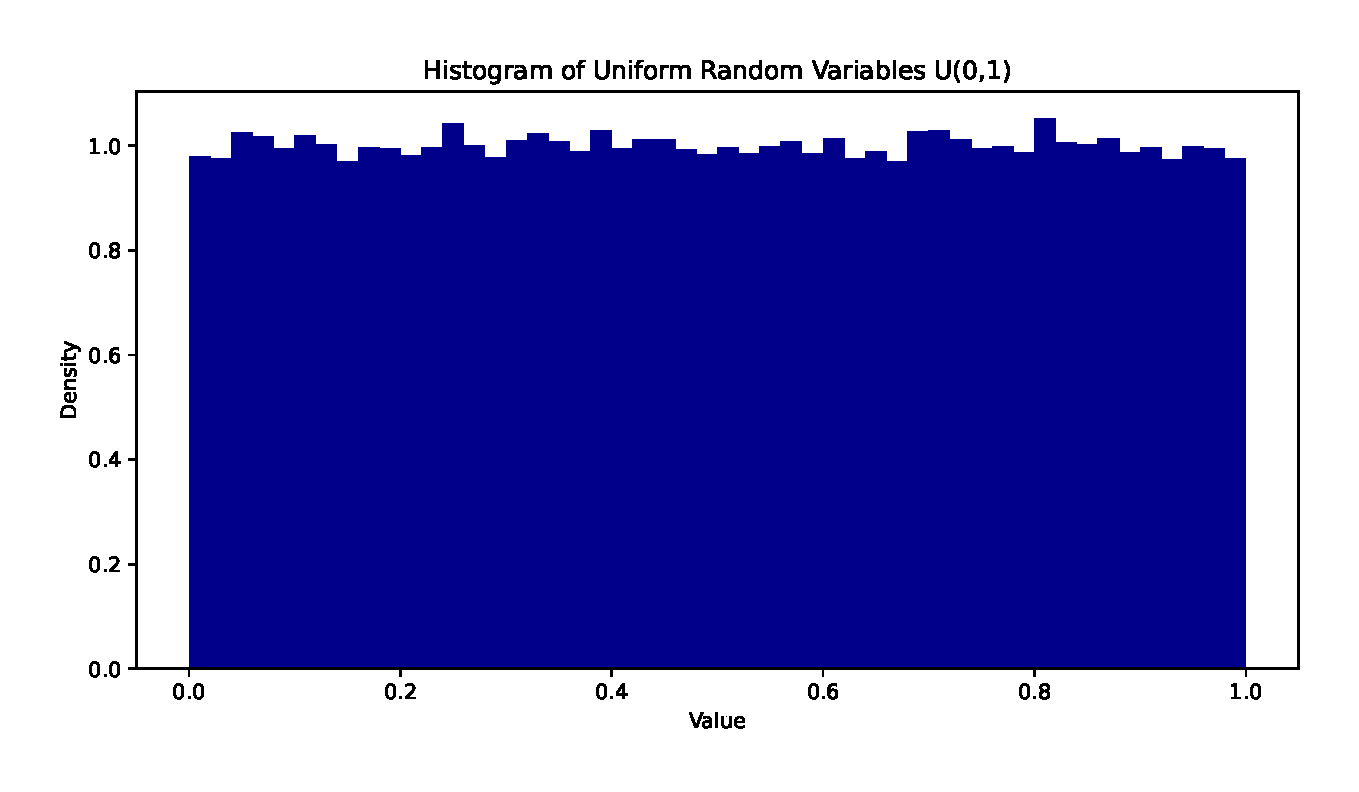
\includegraphics[width=0.95\textwidth]{IMAGENES/ex_2.pdf}
	\caption{Ejemplo de simulación para $n=100000$ muestras.}
\end{figure}

Después de varias simulaciones con diferentes estados iniciales, se puede ver que todas tienen un comportamiento similar al mostrado en la figura anterior, por lo que sí parecen tener una distribución uniforme en el intervalo $[0,1]$.